%#################### 7.1 ####################
\section{Simple pie chart}
	\begin{table}[h!]
	\begin{tabular}{c | c}
	\begin{minipage}[m]{0.4\textwidth}
	\enum{ 
	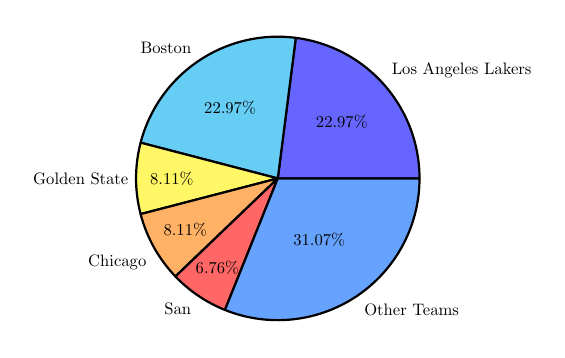
\begin{tikzpicture}[thick,scale=0.6, every node/.style={transform shape}] 
\pie{22.97/Los Angeles Lakers,
22.97/Boston,
8.11/Golden State,
8.11/Chicago,
6.76/San ,
31.07/Other Teams}
\end{tikzpicture}}{7.1}
	\end{minipage}
	&
	\begin{minipage}[m]{0.55\textwidth}
	\renewcommand\textminus{\mbox{-}}%<<<<<<<<<<<
	\begin{lstlisting}[numberstyle=\zebra{red!15}{yellow!15},numbers=left,basicstyle=\footnotesize]{tex}
\documentclass[border=0.2cm]{standalone} 
\usepackage{pgf-pie}  

\begin{document}
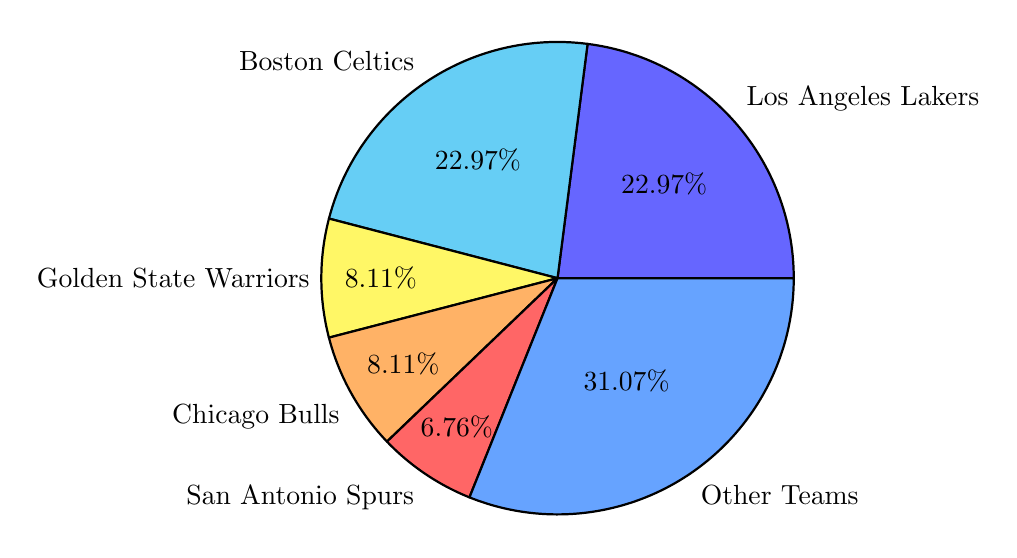
\begin{tikzpicture}
\pie{22.97/Los Angeles Lakers,
22.97/Boston Celtics,
8.11/Golden State Warriors,
8.11/Chicago Bulls,
6.76/San Antonio Spurs,
31.07/Other Teams}
\end{tikzpicture}
\end{document}
	\end{lstlisting}
	\end{minipage}
	\end{tabular}
	\end{table}

	%#################### 7.2 ####################
\section{Circled arrows with text}
\begin{table}[h!]
\begin{tabular}{c | c}
\begin{minipage}[m]{0.4\textwidth}
\enum{ 
\begin{center}
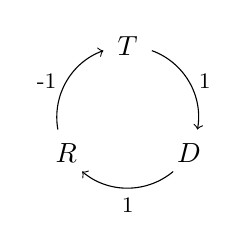
\begin{tikzpicture}[->,scale=.9]
\node (i) at (90:1cm)  {$T$};
\node (j) at (-30:1cm) {$D$};
\node (k) at (210:1cm) {$R$};
\draw (70:1cm)  arc (70:-10:1cm) node[midway, right] {{\footnotesize 1}};
\draw (-50:1cm) arc (-50:-130:1cm) node[midway, below] {{\footnotesize 1}};
\draw (190:1cm) arc (190:110:1cm) node[midway, left] {{\footnotesize -1}};
\end{tikzpicture}\end{center} }{7.2}
\end{minipage}
&
\begin{minipage}[m]{0.55\textwidth}
\renewcommand\textminus{\mbox{-}}%<<<<<<<<<<<
\begin{lstlisting}[numberstyle=\zebra{red!15}{yellow!15},numbers=left,basicstyle=\scriptsize]{tex}
\documentclass{article} 
\usepackage{tikz}

\begin{document}
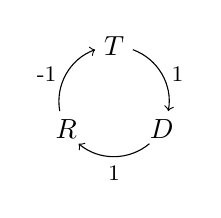
\begin{tikzpicture}[->,scale=.7]
\node (i) at (90:1cm)  {$T$};
\node (j) at (-30:1cm) {$D$};
\node (k) at (210:1cm) {$R$};
\draw (70:1cm)  arc (70:-10:1cm) node[midway, right] {{\footnotesize 1}};
\draw (-50:1cm) arc (-50:-130:1cm) node[midway, below] {{\footnotesize 1}};
\draw (190:1cm) arc (190:110:1cm) node[midway, left] {{\footnotesize -1}};
\end{tikzpicture}
\end{document}
\end{lstlisting}
\end{minipage}
\end{tabular}
\end{table}
\newpage
%#################### 7.3 ####################
\section{Diamond with text}
	\begin{table}[h!]
	\begin{tabular}{c | c}
	\begin{minipage}[m]{0.4\textwidth}
	\enum{   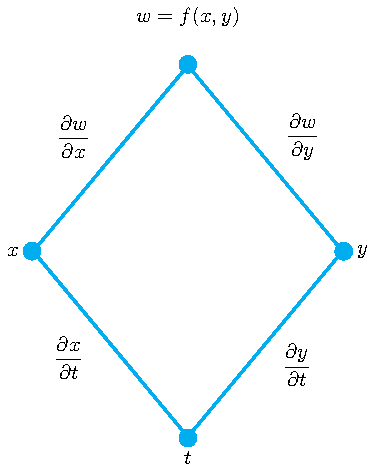
\includegraphics[width=1\linewidth]{7.3.pdf}   }{7.3}
	\end{minipage}
	&
	\begin{minipage}[m]{0.55\textwidth}
	\renewcommand\textminus{\mbox{-}}%<<<<<<<<<<<
	\begin{lstlisting}[numberstyle=\zebra{red!15}{yellow!15},numbers=left,basicstyle=\scriptsize]
\documentclass[a4paper,14pt]{extreport}
\usepackage[left=1.5cm,right=1.5cm,top=1.5cm,bottom=2cm,bindingoffset=0cm]{geometry}
\usepackage{amsmath}
\usepackage{tikz}
\usetikzlibrary{shapes.geometric}
 
\begin{document}
\begin{tikzpicture}
\node[diamond,font=\small,
line width=0.4mm,scale=0.7,
    draw = cyan, minimum width = 7.5cm, %text = red,
    minimum height = 9cm] (d) at (0,0) { };
      \node [above=0.5cm] (a) at (d.90) {$w = f(x,y)$};
      \node [above=0.5cm,right=0.1cm] (b) at (d.45) {$\dfrac{\partial w}{\partial y}$};
      \node [above=0.5cm,left=0.1cm] (c) at (d.135) {$\dfrac{\partial w}{\partial x}$};
      \node [left=0.1cm] (dd) at (d.180) {$x$};
      \node [right=0.1cm] (e) at (d.0) {$y$};
      \node [below=0.1cm] (f) at (d.270) {$t$};
      \node [below=0.9cm,right=-0.3cm] (g) at (d.-30) {$\dfrac{\partial y}{\partial t}$};
      \node [below=0.5cm,left=0.1cm] (h) at (d.220) {$\dfrac{\partial x}{\partial t}$};
      \node at (d.90) [cyan,circle,fill,inner sep=3pt]{};
      \node at (d.180) [cyan,circle,fill,inner sep=3pt]{};
      \node at (d.0) [cyan,circle,fill,inner sep=3pt]{};
      \node at (d.270) [cyan,circle,fill,inner sep=3pt]{};
\end{tikzpicture}
\end{document}
\end{lstlisting}
	\end{minipage}
	\end{tabular}
	\end{table}
%#################### 7.4 ####################
\section{Levels of skills }
\begin{table}[h!]
\begin{tabular}{c | c}
\begin{minipage}[m]{0.4\textwidth}
\enum{   
\skills{{Word/1}}\\
\skills{{\LaTeX/6}}\\
\skills{{C++/2}}\\
\skills{{Python/3}}\\
}{7.4}
\end{minipage}
&
\begin{minipage}[m]{0.55\textwidth}
\renewcommand\textminus{\mbox{-}}%<<<<<<<<<<<
\begin{lstlisting}[numberstyle=\zebra{red!15}{yellow!15},numbers=left,basicstyle=\scriptsize]{tex}
	\documentclass{report}
	\usepackage[T1]{fontenc}
	\usepackage{tikz}
	\usepackage{xcolor}

	\definecolor{white}{RGB}{255,255,255}
	\definecolor{gray}{HTML}{4D4D4D}
	\definecolor{maingray}{HTML}{B9B9B9}

	\newcommand\skills[1]{ 
	    \begin{tikzpicture}
	        \foreach [count=\i] \x/\y in {#1}{
	            \draw[fill=maingray,maingray] (0,\i) rectangle (6,\i+0.4);
	            \draw[fill=white,gray](0,\i) rectangle (\y,\i+0.4);
	            \node[above right] at (0,\i+0.4) {\x};
	        }
	    \end{tikzpicture}
	}

	\begin{document}
	\skills{{b/2}}
	\skills{{a/1}}
	\end{document}
\end{lstlisting}
\end{minipage}
\end{tabular}
\end{table}
%#################### 7.5 ####################
\section{Levels of skills }
\begin{table}[h!]
\begin{tabular}{c | c}
\begin{minipage}[m]{0.4\textwidth}
\enum{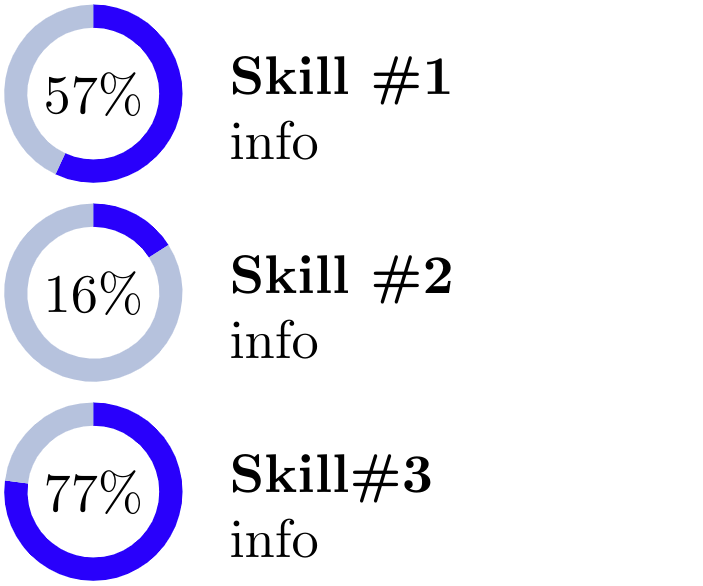
\includegraphics[width=1\linewidth]{7.5.png}}{7.5}
\end{minipage}
&
\begin{minipage}[m]{0.55\textwidth}
\renewcommand\textminus{\mbox{-}}%<<<<<<<<<<<
\begin{lstlisting}[numberstyle=\zebra{red!15}{yellow!15},numbers=left,basicstyle=\scriptsize]{tex}
\documentclass[svgnames]{article}
\usepackage{tikz}
\usetikzlibrary{calc}
\usepackage{siunitx}% only to force percentages to be integers
\usepackage{enumitem}

\let\realItem\item% save for later use
\newcommand\percentageItem[1][10]{%
  \realItem[\smash{\tikz[baseline];
    \draw[thick,line width=1.5mm,Blue](90:5mm)
          arc [radius=5mm, start angle=90, delta angle=-#1*3.6];
    \draw[thick,line width=1.5mm,LightSteelBlue](90-#1*3.6:5mm)
          arc [radius=5mm, start angle=90-#1*3.6, end angle=-270];
    }}]%
}
\newlist{achievements}{itemize}{1}
\setlist[achievements]{
  before=\let\item\percentageItem,%make \item = \percentageItem
  leftmargin=*,
  label={},
  itemsep=3mm,
}

\begin{document}

\begin{achievements}
  \item[57]\textbf{Skill \#1}\\info
  \item[16]\textbf{Skill \#2}\\info
  \item[77]\textbf{Skill \#3}\\info
\end{achievements}

\end{document}
\end{lstlisting}
\end{minipage}
\end{tabular}
\end{table}
%#################### 7.6 ####################
%#################### 7.7 ####################
%#################### 7.8 ####################
%#################### 7.9 ####################
%#################### 7.10 ####################
%#################### 7.11 ####################














